%---------------------------------------%
%           P R E A M B L E             %
%~~~~~~~~~~~~~~~~~~~~~~~~~~~~~~~~~~~~~~~%


% Package configuration
%\PassOptionsToPackage{biblatex}{style=ieee, backend=biber}
%\PassOptionsToPackage{glossaries}{}


% Document Class ===============================================================
\def\PathToTumTemplate{.}
\PassOptionsToClass{ebook}{tum_thesis}
\documentclass[%
    %ebook   % create digital ebook
    ]{\PathToTumTemplate/thesis/tum_thesis}



% thesis settings
% -------------------------------------------------------------------
\RequirePackage[english]{babel}   % or 'ngerman', delete .aux after changeing




% thesis information
% -------------------------------------------------------------------
\title{TODO rename}                          % defines \thetitle
\author{Márton Donát Nagy}                         % defines \theauthor
\myemail{mdonat.nagy@tum.de}                 % defines \theemail
\authorsaddress{Musterstr. 42 \\ 42424 Musterstadt}
\studentnumber{00000000}


\doctype{Master's Thesis}
\professor{Prof. Dr. phil. nat. Sebastian Steinhorst}
\advisor{Adam Advisor}
\coadvisor{Corinna Coadvisor}
\submitdate{\today}



% chair information
% -------------------------------------------------------------------
\RequirePackage{\PathToTumTemplate/tum/ei/esi/esi}  % your chair
\RequirePackage{\PathToTumTemplate/tum/tum_header} 
\logoheader{\vspace*{-3cm}\printTumHeader}


% listing language
\lstset{ language=ada }

% other packages
% -------------------------------------------------------------------
\RequirePackage[automake=true, toc, acronym]{glossaries}
\setacronymstyle{long-short}
%\makenoidxglossaries
\makeglossaries
\RequirePackage{listings}
% \begin{lstlisting} 
% 	code here...
% \end{lstlisting}
\RequirePackage{graphicx}
% \includegraphics[width=\columnwidth]{img/uml_spec}
\RequirePackage{siunitx}
% \SI{3.14}{\meter\per\second}
\RequirePackage{microtype}          % improved kerning, layout
\RequirePackage{hyperref}           % clickable references
\RequirePackage{booktabs}           % professional tables
\RequirePackage{caption}


% use \emph{} for special terms, use \texttt{} for general code variables, and \lstinline{} for code.
% use \textbf{} for heading cells in tables
% use \mathrm{} in math environment for things that are not variables, like function names.
% use \SI{3.14}{\meter\per\second} for physical quantities (requires \RequirePackage{siunitx})
% use \gls{RAM} for acronyms. This feels annoying but will take care of everything and allows you to copy paste text without worrying.


% abbreviations / acronyms
% -------------------------------------------------------------------
\newacronym{ctai}{CTAI}{Claim Truth Assessment Inaccuracy}
%\newacronym[shortplural={BLKs},longplural={Belastungskollektive}]{BLK}{BLK}{Belastungskollektiv}
\newacronym{trsys}{TR System}{Trust and Reputation System}
\newacronym{rs}{RS}{Reputation System}
\newacronym{ts}{TS}{Trust System}

% glossary entries
% -------------------------------------------------------------------
\newglossaryentry{ex}
{
	name={sample},
	description={an example}
}
\newglossaryentry{scenario}
{
	name={scenario},
	description={Description of a complete simulation environment for Pyrepsys. Specifies the reputation scheme, improvement methods, agents, possible review values etc. See section~\ref{sec:scenario} for details.}
}
\newglossaryentry{claim}
{
	name={claim},
	description={TODO}
}
\newglossaryentry{review}
{
	name={review},
	description={TODO}
}
\newglossaryentry{author_review}
{
	name={author review},
	description={TODO}
}
\newglossaryentry{gr_truth}
{
	name={ground truth},
	description={TODO}
}
\newglossaryentry{score}
{
	name={score},
	description={TODO}
}
\newglossaryentry{claim_probability}
{
	name={claiming probability},
	description={A percent likelihood determining whether an agent initiates a claiming process if given an opportunity. Specified in scenarios for each agent.}
}
\newglossaryentry{main_rng_chain}
{
	name={main random chain},
	description={TODO}
}
\newglossaryentry{measured_claim_score}
{
	name={measured claim score},
	description={TODO}
}
\newglossaryentry{claim_range}
{
	name={claim range},
	description={TODO}
}
\newglossaryentry{distort_strategy}
{
	name={distortion strategy},
	description={TODO}
}
\newglossaryentry{rate_strategy}
{
	name={rating strategy},
	description={TODO}
}
\newglossaryentry{distorted_claim_quality}
{
	name={distorted claim quality},
	description={TODO a value produced by the distort strategy from the measured claim q}
}



% glossary and acro usage
% -------------------------------------------------------------------
% \gls{maths} \glspl{formula} Gls Glspl to capitalize
% \acrlong{gcd}, \acrshort{gcd} \acrfull{lcm} \~pl()



% document begin (output starts here)
% -------------------------------------------------------------------
\begin{document}
\frontmatter

% titlepage
\maketitle

% Colophon
\newcommand{\thecolophon}{  
    \begin{colophon}
        \vspace*{1cm}     
        \begin{minipage}{0.5\textwidth}\begin{flushleft}
        This thesis was typeset using the XeTeX{} 
        typesetting system developed by Jonathan Kew. 
        \end{flushleft}
        \end{minipage}
    \end{colophon}
}
%\thecolophon   % uncomment to print colophon (optional)
%\cleardoublepage


% declaration
\begin{authordecl}
    \noindent I, \theauthor, declare that this thesis titled
    ``\thetitle'' and the work presented in it are my own unaided
    work, and that I have acknowledged all direct or indirect sources as
    references.

    This thesis was not previously presented to another examination board
    and has not been published.

    \vspace{2em}

    \noindent Signed:\\\vspace{1em}
    \noindent\rule[0.5em]{25em}{0.5pt} % This prints a line for the signature
     
    \noindent Date:\\\vspace{1em}
    \noindent\rule[0.5em]{25em}{0.5pt} % This prints a line to write the date
    \rmfamily
\end{authordecl}
\cleardoublepage


% abstract
%Abstract: Short summary of the context, the problem, your approach and its experimental results (numbers!).
\begin{abstract}
    This thesis is about ...
    This thesis shows that ...
\end{abstract}



% table of contents
\setcounter{tocdepth}{1}
\tableofcontents



\cleardoublepage
\mainmatter


% CHAPTER ######################################################################
\chapter{Introduction}
% ##############################################################################
%Introduction: Draw a picture of the context which your work is embedded.
%    Motivation: Describe the ultimate goal, the glory future that we want to reach.
%    Problem Statement: Why is there currently a gap between us and our goal? Why is SotA not sufficient? What is the problem?
%    Contributions: What will you do / have you done to narrow this gap? List 3-5 contributions as bullet points.
 
 
\lettrine{T}{echnology} is on the move and this topic is important because it will change the world.




% --------------------------------------------------------------
\section{Problem Statement}\label{sec:probstat}
% --------------------------------------------------------------
As a long term goal we would like to have ...
The problem is that ... still does not work. So we will investigate the questions
\begin{itemize}
    \item whether A
    \item or whether B
\end{itemize}



% --------------------------------------------------------------
\section{Scenario}
% --------------------------------------------------------------

The scenario and assumptions and the background of this thesis. We assume ..., we will focus on ... and we will exclude ...

%TODO describe the hypothetical example scenario of the autonomous driving within intersection management, cars estimating ETA etc. Let know that it will be used throughout the thesis to illustrate concepts and help define goals, the direction solutions, approaches go.
on a more broader sense, the work is intended to be general enough that it could be applied for other iot/cps type applications as well


% --------------------------------------------------------------
\section{Task Definition}
% --------------------------------------------------------------

We will do

\begin{itemize}
    \item try A
    \item try B
\end{itemize}



% --------------------------------------------------------------
\section{Structure of This Document}
% --------------------------------------------------------------

First, ...



% --------------------------------------------------------------
\section{Terminology}
% --------------------------------------------------------------
% TODO: place this somewhere else, maybe not a full section for it
describe user, peer, agent, principal, node etc namings
in research used according to domain of the paper

network

underlying value, trueness, ground truth, 

reputation score, estimate, global rating

rating, opinion, review

Content, transaction, service, product, file, claim

advisor, witness, second hand reputation


internal vs agent-exposed: in the program, internal is how reputations, reviews, claims etc are stored and refers to [0,1] real
agent-exposed is how the agent sees everything, typically [1,9] and discrete integers
in the code \_i vs \_ae denotes which type a variable stores


score: review value, claim value, reputation etc. referred generally







% CHAPTER ######################################################################
\chapter{State of the Art}\label{chap:sota}
% ##############################################################################
%State of the Art (SotA): Where is technology right now? How does it work? How does it relate to your work?

\lettrine{T}{his} chapter gives an overview of ... 


% --------------------------------------------------------------
\section{Domains of Trust and Reputation Research}
% --------------------------------------------------------------
% TODO not necessarily a full section, also not here

discuss fields like WSN, p2p filesharing, MAS, mobile sensor systems, flying ad hoc networks, vehicular ad hoc networks, ecommerce, recommendation systems online stuff like imdb or hotel ratings....


% --------------------------------------------------------------
\section{Evaluation and Comparison}\label{sec:sota_eval}
% --------------------------------------------------------------

\subsection{Theoretical Categorization}

\subsection{Simulation Frameworks}


\cite{zhang_detailed_2008} does an ad hoc comparison of accuracy improvement / unfairness filtering methods. Maybe mention


\subsubsection{Asd Example}



% --------------------------------------------------------------
\section{Improvement Techniques for Reputation Systems}\label{sec:sota_nolink_todo}
% --------------------------------------------------------------
% TODO other name: accuracy , robustnesss

Various papers propose methods to make reputation systems more robust against exploitations and improve the accuracy of their reputation calculation. Works with this goal are most commonly in the e-commerce and online recommendation systems domains. A smaller amount also explore other domains. 


\subsection{Categorization}

accuracy (better function) vs attack countering
they can overlap

categories based on domain 
mentioned, but not the main driver of categorization here, because looking for general ideas to implement in IoT etc as cross domain
better if domain dependent or independent

based on general idea
primary categories for this collection

endo vs exogenous
mention that it gained some traction in research
Whitby et al. group methods to identify and remove unfair ratings into two categories: endogenous and exogenous approaches \cite{whitby_filtering_2014}. Endogenous refers to methods where only the rating values are analyzed for statistical anomalies. Exogenous methods consider factors other than the ratings themselves for detecting unfair ratings. Such external factors are for example the reputation of the rater, in which case the assumption is that low-reputation users are more likely to give unfair ratings.

Endogenous could be expanded or generalized to say only the ratings, reviews, feedbacks, including their value and accompanying text, any data and metadata are analyzed.

\cite{zhang_detailed_2008} uses apart from the endo-exo categorization two other categories: public-private and global-local. These are adopted specifically for e-commerce-type scenarios where local trust (past experiences) and local advisor opinions both play a role.

Public and private differentiated between how advisor opinions are judged for trustworthiness.
in private methods, agents evaluate an advisor's opinion based on whether past opinions received by the same advisor turned out to be correct or not. Data for evaluation is limited to the specific advisor's interactions with the specific agent in the past.
in public methods, agents judge advisors based on the advisor's ratings across the whole system in the past. Here, all previous opinions of the advisor and their subsequent results are taken into account, not just that which were provided for the agent currently doing the evaluation.

local refers to methods where looking for received unfair ratings of an agent is based on all the ratings that agent received, but not other agents. (E.g. this seller typically gets 4..5 so this 1-rating is suspicious) In a sense, opinions are isolated between agents.
in global methods, advisor (interchangeable with rating, feedback, review etc...) trustworthiness is judged using ratings on all the agents in the system.


Although defined for e-commerce advisor-opinion scenario, these categories can be understood in a more general sense. In this case, sellers are to be understood as agents providing content (data, service, product, sensor reading...) and receiving a rating. Vice versa, buyers are receiving the content and providing the rating. Advisor refers to any third party contributing to the final aggregated reputation (rating, trust level) of a potential transaction partner. Opinion is any rating, review or feedback in a more broader sense.

The public-private and local-global distinction can be understood as two sides of the transaction. In public-private, the rater is judging, 

They also identify 4 capabilities a complete improvement approach should have:
-majority: work if majority is unfair / malicious
-flooding: function under sudden onset of ratings in short time
-lack of experience: still work when agents don't have any connections or private XP
-varying: agent behavior change should not pose a problem

reactive or proactive. The reactive solutions intend to identify the unfair feedbacks and the proactive solutions propose incentive to the buyers to encourage them to report fair feedbacks \cite{thakur_reputation_2019}





Accuracy of ratings is a crucial part of any reputation system. This is true whether transactions or directly the users are rated. 
Many attacks exploit exactly this vulnerable point of TRs. Slandering, promoting and other attack strategies, see attacks chapter...

Interpreting accuracy of ratings is difficult in systems where people rate based on their subjective experiences, or where there is a degree of uncertainty. E.g. e-commerce rep systems
Since ratings in real-life situations are not accurately computable
analogous term is honesty of users. some researchers (cite?) use a scale based on honesty to categorize users from purely malicious to purely honest. In this case this refers to given feedback, as other dimensions of "inhonesty" is also possible, like malice in transaction content. There was a paper that categorized malice into these two ways, cite mayb. Also this discussion mayb not here.

Accuracy's further interpretation is a sort of "trueness" value. This implies that an objectively true and absolutely accurate rating of a user's experience exists.
This is then different from the feedback the user gives into the system.
The user may or may not be aware of this "true rating." If not aware, maybe bias, subjectively very unpleasant experience. Some call this inherent bias. E.g. e-com the product is perfect but shipping time was bad and gives a 1-star rating. 
(There is a philosophycal aspect to this, as this is saying "you experienced this a 1/5 but we say it really was a 4/5" and what right or objective measure exists to permit this.)
If the user is aware of the "true quality," giving a doctored rating out of malicious intent is still a possibility. 
In any case, the result is that the given rating differs from a hidden, "objectively true" rating. This situation is called an "unfair" rating by Josang.

Some other metrics measuring accuracy exist in evaluation frameworks. See chapter metrics.


(continuation of above) machine populated reputation systems where ratings are given by algorithms evaluating data, are more fitting to calculations of numerical accuracy



\subsection{Statistical Reputation Systems}

The Whitby et al. work with this line of thought in their paper in \cite{whitby_filtering_2014}. 
they extend the BRS from a previous paper
They argue that unfair and fair ratings have different statistical patterns. Consequently, it is possible to identify and filter unfair ratings with statistical methods.
% TODO expand on explanation


TRAVOS is a bayesian trust and reputation method based on the beta probability distribution \cite{teacy_travos_2006}. It uses both experience-based local trust and global reputation, depending on whether past experience with a particular transaction partner is available or not. If a potential transaction partner is not already well known, the system relies on global reputation reported by third party advisors. Deception from advisors is countered by evaluating the perceived accuracy of their past opinions. Specifically, first a probability is calculated for how likely it is the third party advisor gives an accurate opinion. This is done on the basis of previous opinions given, and the eventual outcomes of those transactions. Then as a second step, the opinions likely to be inaccurate are altered so as to have a smaller impact on the final calculated reputation. This is done through decreasing the parameters of the distribution which represents the advisor's opinion. An opinion modified in this manner will influence the expected value of the final reputation distribution to a lesser degree.

TRAVOS and the Beta Reputation System are very similar. They are both bayesian statistical methods using the beta probability distribution. However, the Beta Reputation System does not differentiate between direct observarions and advisor recommendations. Additionally, the two methods handle inaccurate (unfair, malicious...) ratings differently. TRAVOS is an exogenous approach, scrutinizing each individual advisor based on the perceived accuracy of their past opinions. BRS is an endogenous approach, taking a single rating and judging it based on how far it is from the mainstream opinion.


There is the question of what to do with opinions caught in the filter. Completely disregard, lower weight, or temporarily disregard...

Majority opinion methods rely on the assumption that the majority of the users are honest and accurate.



The Dirichlet Reputation System is worth mentioning as a multinomial generalisation of the Beta Reputation System \cite{josang_dirichlet_2007}. Using the dirichlet distribution instead of the beta distribution allows more than two discrete rating levels. It is a method well grounded in bayesian statistics, and is built around similar concepts to the BRS. Specifically, aging of ratings is also present. A similar extension for filtering non-majority outlier opinions like in the BRS was not found for the Dirichlet Reputation System.


The Personalized Approach introduces in \cite{zhang_personalized_2006} ...
in e-com, private opinion and global reputation of advisor both used, agents can weight these two, has aging, private: agent take opinion giver, see how they rate commonly rated fourth parties, public reputation based on how consistent the advisor's rating of other parties is

\cite{yu_detecting_2003} Weighted Majority Algorithm 
advisors given a weight to sum their opinions, if incorrect based on future transaction, the weight is decreased, constantly wrong advisors are thus filtered eventually

The authors of \cite{zhang_personalized_2006} and \cite{zhang_detailed_2008} take a survey of previous improvement methods, introduce a new method (personalized approach) and compare them, including experimental measurements. The methods compared are the Beta Reputation System, TRAVOS, Personalized Approach, Bayesian Network Approach and Weighted Majority Algorithm. 

\cite{iltaf_mechanism_2013}
"based on the assumption that a dishonest recommendation is one that is inconsistent with other recommendations and has a low probability of occurrence in the recommendation set. Based on this assumption, a new dissimilarity function for detecting deviations in a recommendation set is defined"

\cite{zakirullah_detection_2014} in MANETs, dissimilarity function based

\cite{rezvani_randomized_2020} uses randomly selected samples of all reviews to calculate global reputation. (e-com)

\cite{baby_secure_2014} uses a five-step process to make the reputation system more secure against unfair ratings:
Evaluation based filtering, 
Time domain unfair rating detector, 
suspicious user correlation analysis, 
trust analysis based on Dempster-Shafer theory and 
malicious user identification and reputation recovery.

\cite{ngo_survey_2007} also surveys methods against unfair ratings. Considered approaches are
filtering based on majority opinion (Whitby et al), 
entropy-based filtering, 
reputation trees, (agents reputation is their rating's weight)
controlled anonymity and agent clustering,
clustering ratings and checking IP address, 
using trust rating in MANETs and 
WMA and belief function.

\cite{azzedin_identifying_2010}

"Transactions are evaluated by both the source peer and the target peer in [9]. A source peer's feedback is considered
consistent if it agrees with the target peer's self-evaluation. Assuming most of the peers are trustworthy and honest,
most inconsistencies would be in the case that the source peer reports a trustworthy transaction as untrustworthy
(badmouthing) or an untrustworthy transaction as trustworthy (collusion to boost the target peer's reputation). Thus,
a source peer is suspected to be providing false feedbacks if the proportion of inconsistent feedbacks exceeds certain
threshold, T. Feedbacks from inconsistent peers are no longer accepted.
" WARNING, this is a quote of consistency based

"The reputation system in [15] uses a measurement called credibility factor. The credibility factor increases if a
recommender provides a recommendation that matches the actual result of the transaction. From the credibility,
discredibility factor can be derived. A recommender whose discredibility factor is higher than its credibility factor
will be filtered out."
WARNING quote of credibility based

\cite{dellarocas_immunizing_2000} for e-com, introduces two extension ideas to TRs to combat unfair ratings:
controlled anonymity to avoid unfairly low ratings and negative discrimination
cluster filtering to reduce the effect of unfairly high ratings and positive discrimination

\cite{margaris_improving_2017}\cite{margaris_improving_2018} work with the idea of normalizing the rating scale each agent is typically using. This approach comes from collaborative filtering systems.

\cite{zupancic_qade_2015}
"finds similar agents and consider them as reputable source of information. Further, the agents compare their trust values with trust values of similar agents"



%TODO this part obv not here, rather in approach
explicit inclusion of private experience as a system component
possibility of maintaining a trust network and getting recommendations (opinions) from them as advisors

both of these are done in a system primarily used by men. e.g. in e-commerce, once the reliability and quality of a provider is known through first-hand experience, reviews and ratings are not scrutinized as they would be by first-time buyers. Social proof mechanisms like getting recommendations and opinions from friends or trusted contacts is also very common without it needing to be part of any reputation system. 

This is different in reputation systems made for and used by algorithmic agents. whether decisions are made by other machine agents or the system (algorithm) itself like in a traffic management scenario, it will only ever consider factors it was programmed to. There is a case for explicitly integrating these human mechanisms or similar methods inspired by them. The potential upside is better reputation estimate accuracy, or at the least better decision outcomes. On the other hand, the increased complexity provides new attack vectors and thus potentially enables new exploits.

Mechanisms like a list of trusted "friends," trust networks, third party advisors providing private opinions come from a trust-centric approach to the decision making problem. Three separate categories give themselves from this distinction: pure reputation systems, reputation systems infused with trust components and pure trust systems. Only the first two is of interest within the scope of this thesis.

With this, the categorization of local-global and public-private is also easier to define in a broader context.





Provide incentives to prevent or mitigate unfair ratings: 
\cite{thakur_reputation_2019}
\cite{jurca_minimum_2006}

\cite{liu_reputation_2015} recovers the temporary damage of sellers who were given a lower rating by a buyer by mistake, and the buyer willingly corrects it. The seller's reputation is temporarily inflated to revert reputation damage.

\cite{wan_context-aware_2012} aims to improve unfair rating detection by analyzing selected factors of the environment the detection is deployed in and selecting the most suitable approach from a multitude of methods. 

learning approaches:
\cite{khoshkbarchi_coping_2017}
\cite{wang_bayesian_2003} Bayesian Network-Based Trust Model, p2p, reinforcement learning
\cite{yazidi_solving_2017}
%TODO more 

approaches combining first hand trust observations with reputation in some way:
\cite{boudec_robust_2003} for manets, everyone maintains a first-hand reputation (i.e. trust) and a second-hand (global) reputation of others. First-hand reputation is exchanged by nodes occasionally, and data is combined to reach a better accuracy. The system employs aging and occasional re-evaluation to enable reputation redemption.
\cite{huynh_handling_2005}
%TODO mroe

regarding recommender systems:
\cite{hutchison_combining_2013}

% --------------------------------------------------------------
\section{Attacks and Exploits}\label{sec:sota_attacks}
% --------------------------------------------------------------






% CHAPTER ######################################################################
\chapter{Approach}\label{chap:approach}
% ##############################################################################
%Materials, Methods, Models, Algorithms, or Tools: Explain what the reader needs to understand in order to understand your approach.
%    Which existing methods and tools will you use to approach the problem?
%    What is your system model? What are your assumptions? 

%Approach: Explain your concept to solve the problem.
%    Intuition first: Give a short, informal description of your idea using a simple diagram and/or a simple example.
%    Architecture/Model: Fully describe your approach on a conceptual level without giving details that belong to only one possible implementation.
%    Example: Write “We need a hash function with the following properties.” NOT “We need/use SHA-256”


%TODO somewhere in this chapter, discuss how in ecom or other domains its a problem that not many ratings are given, while in fully machine populated it can be mandated to leave a review. then again its a question of who's in sensing distance e.g. in the intersection management case






% --------------------------------------------------------------
\section{Improving Reputation Estimates}\label{sec:estimate_improvements}
% --------------------------------------------------------------
% other names: Robustness, Accuracy, Trueness

\subsection{Categorization}

other cateogry: what is rated


agents 
content
links
could call this rating dimension aka who/what is rated exactly
can represent as graph (vertices, edges, directed boxes as content)
discuss special cases, e.g. in e-com, rating the very same physical products between different sellers, an extra rating dimension is neede for service quality (packaging, mayb its white/gray label, shipping time, customer service interaction's quality etc... this is different than the product rating and also diff from the agent rating itself
also accuracy rating


\subsection{next todo}

there is a case to be made about applying improvement techniques depending on the environment of the reputation system. e.g.

rating aging makes sense only if behavior are known to change over time. if for sure constant (like machines which receive no updates whatsoever) then it has no point

frequency of feedback rating given after transaction.. means only something maybe if its not mandated, which in a fully machine network might as well just be

outlier filtering makes sense only if you know that significant (extreme) differences in transaction experiences are unlikely to the point that such claim becomes suspicious. Once highly subjective experiences come into play, it is wrong to say a nonmajority opinion is unfair. Or in a highly dynamic agent population, where behavior changes often and rapidly, extremity filtering is contraproductive since it introduces reputation lag.



differenciate based on how many ratings contributed to a final reputation score, i.e. confidence. like if a new entrant gets a default of 4, and another has 4 based on a 1000 ratings, this difference should be noticable and agents should be able to make decisions based on that

\subsection{Outlier Filtering based on Majority Opinion}
%other name: filtering approaches, extreme outlier filtering

\subsection{Aging Ratings}

\subsection{Normalizing Rating Range}
% Normalizing to counter strictness/leniency

\subsection{Weighing based on Rater Reputation}

\subsection{Anonymous ratings}


outlier filtering based on something: statistical, entropy, dissimilarity function, similarity
dis/similarity is also a kind of stereotype-based TR, also collaborative filtering ties in here
normalizing rating range
weighing based on rater reputation
anonymous ratings
adding local trust
use random subsets to calculate reputation
Weighted Majority Algorithm 
simplifying rating space (some believe that +- or only + or - helps eliminate attacks)
feedback consistency-like solution -- in intersection, car estimates ETA, later rates its own ETA, and see if others rate the same ETA consistently -- inspired by one menitoned in \cite{azzedin_identifying_2010}

pair ETAs with uncertainty (generally: stake)
if I can say along with the claim how sure i am in the claim
or maybe once when I commission a car, I can say how accurate the sensor reading is, so this accuracy rating remains static for a long time
then if this uncertainty is larger, I have more room to manipulate the ETAs within plausible deniability, but on the other hand the other cars can say my claim is more worthless because I have a large uncertainty range..

%TODO sota list techniques and categories, no all-encompassing categorization exists so this'd go into approach

also in this part: author reviews




% --------------------------------------------------------------
\section{Pyrepsys Evaluation Framework}\label{sec:approach_evaluation_framework}
% --------------------------------------------------------------
% aka. Simulation System

check how to implement these
can use existing eval frameworks? or need own one in python
if latter, what components
a diagram can be good also for the presentation



The Pyrepsys Reputation System was designed in order to allow simulation, comparison and evaluation of selected reputation schemes with various environment conditions. 
This chapter gives a conceptual introduction for Pyrepsys, including main design goals, simulation flow and core features.
For a description of the concrete implementation of Pyrepsys, see Chapter~\ref{chap:implementation}.

Overall requirements and unique approaches warranted the inception of a new reputation simulation framework. 
These are among others:
\begin{itemize}
    \item domain-independence
    \item the use of one or more reputation imporvement methods
    \item ability to represent \glspl{claim}
    \item possibility of second-order rating schemes like stakes
    \item full simulation of agents
    \item flexible review values (to support custom integer ranges)
    \item extendability and ease of modification for fast prototyping
\end{itemize}


\subsection{Design Goals}
\subsubsection{asd}
Flexibility and extendability are among the main design objectives of pyrepsys.
Variables can be altered in scenario configuration files.
The size and composition of the agent population is customizable.
New agent behaviors, metrics, reputation calculation and imporvement methods can be easily added.





Pyrepsys is a one-stop solution for simulating, comparing and evaluating reputation schemes.
Simulation of scenarios is performed on a round-by-round basis.
Shared configuration among scenarios, simulating batches of scenarios in succession and controlled random number generation help compare different scenarios.
Evaluation is aided by metrics.
These can automatically generate graphs and export data from simulations.



Miscallaneous supportive functionalities are also discussed in this chapter.
A scenario configuration creator can be used to make a batch of scenarios with variations along selected configuration parameters.
Extensive automated self-testing can verify the integrity of the simulation framework if any changes are made.
Finally, profiling and benchmarking tests are provided to identify simulation bottlenecks and measure performance.


\subsection{Scenarios}\label{sec:scenario}
A \gls{scenario} is the description of a complete simulation environment including reputation schemes and agents with various behaviors.
All parameters that are followed during the simulation are part of the scenario.
Some of the most important are listed below.

\begin{itemize}
	\item how reputation values are calculated
	\item which reputation improvement methods are applied
	\item the size of the agent population
	\item how agents behave during simulation
	\item how long the simulation goes (i.e. how many rounds)
	\item the possible rating and reputation values (e.g. binary, integers 1 to 5)
	\item what seed is used to generate random numbers
	\item what graph and data exports metrics should be created
\end{itemize}

In this way, a scenario encapsulates all that is in a single simulation.
This helps organizing combinations of simulation parameters and comparing them.
For example, when the goal is to see what effect malicious agents have, one could draft separate scenarios with varying percentage of malicious agents ranging from 0\% to 100\% in each.

In the Pyrepsys implementation, it is possible to describe scenarios without a full specification.
This means not all needed parameters are listed, just some selected ones.
In this case, the missing parameters are taken from a default scenario configuration.
This is useful when the effect of one or more parameter changes are needed, since those can be simply listed alone in their scenario configuration.
This is described along the implementation in chapter~\ref{chap:implementation}.
For all conceptual discussions, a scenario refers to all the simulation environment fully specified, regardless of where they come from in the implementation.


\subsection{Simulation Flow}
Simulation in Pyrepsys is built around \glspl{scenario}.
Each invocation consists of simulating one or more scenarios after each other.
At the beginning, the default scenario configuration is fetched.
Then Pyrepsys reads and applies the individual configuration for each scenario.
The scenario is simulated after these preparations.
Once all scenarios are finished, the results processor module exports collected data and draws graphs based on the selected metrics.
The simulation part's schematic flow is shown in figure~\ref{fig:simulation_flow}.

Scenario simulation is performed on a round basis.
The number of rounds is part of the scenario configuration.
Each round consists of four distinct phases:

\begin{enumerate}
	\item claiming
	\item rating of new claims
	\item applying reputation improvements
	\item reputation calculation
\end{enumerate}

\subsubsection{claiming}
Claiming is the part where agents can make new \glspl{claim}.
During this phase, all agents get an opportunity to make one new claim.
Whether an agent ends up publishing a claim or not depends on multiple factors.

First of these is the agent's \gls{claim_probability}.
This represents the likelihood of them attempting a claim if given an opportunity.
A more consumer-type agent would have a lower probability and thus claim rarely if ever.
On the other hand, producer-type agents would tend toward higher probabilities, and claim more often.
The random check whether agents attempt a claim or not is performed on the \gls{main_rng_chain}.

If the agent passes this check, a claiming process begins.
First, a claim is generated containing a random \gls{gr_truth}. 
The ground truth is not directly accessible for the agent.
It can however be measured, which is the second step of the claiming process.
Measurement results in the \gls{measured_claim_score}, which represents an approximation of the claim's true quality.
How good this approximation is, depends on the agent's ability to assess claims.
Further details of measuring claims is described in section~\ref{sec:approach_measure_claim}.

With the measured truth, the agent executes its \gls{distort_strategy}.
It essentially applies one of the distortion methods found in section~\ref{sec:distort_strategies}.
The resulting value is the \gls{distorted_claim_quality}.

At this point the agent checks whether the distorted quality falls in the agent's \gls{claim_range}.
Claim range serves as a minimum and maximum limit as to what claims an agent is willing to publish.
If the distorted claim quality falls outside these limits, the claim is discarded and claiming is aborted.
In this case, the agent will not claim in this round.

If the limits are not violated, the new claim will be published.
As a last step, the agent creates an \gls{author_review}.
\Glspl{author_review} are special \glspl{review} appended to each claim by the claiming agent, the author.
The review value is always the distorted claim quality from the previous step.

- idea of author review
- what each thing represents
  - accuracy is the agents competency "expertness" / unwilling inaccuracy
  - distortion is honesty / willing inaccuracy
  - author review is a declaration on what the claimer thinks his claim is worth

TODO continute from here

\gls{claim_range}
\begin{figure}[]
  \begin{center}
        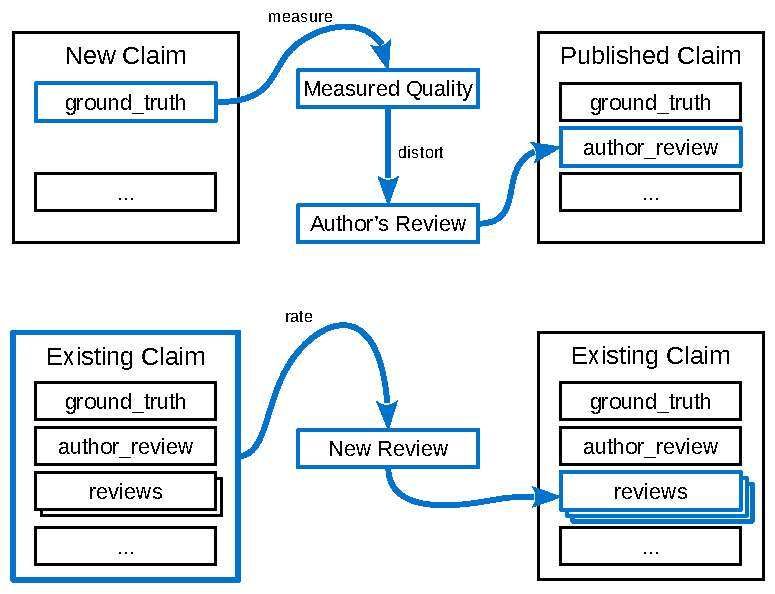
\includegraphics[width=1\linewidth]	{../images/claim_rate_process-crop.pdf}
    \caption{
    Schematic representation of claiming (above) and rating (below) processes with the involved claims and reviews.
	\emph{Claiming} (above) spawns a new claim without any reviews, containing a random \gls{gr_truth}.
	The claimer agent measures this hidden quality and distorts it, resulting in a value representing the clamer's opinion of his own claim.
	This is attached as an \gls{author_review} to the claim to be published.
	\emph{Rating} (below) takes an existing published claim.
	The rater agent takes all data relevant to the claim and produces a \gls{review}.
	This is then appended to the other reviews on the same claim.
    }
    \label{fig:claim_rate_process}
  \end{center}
\end{figure}




\begin{figure}[]
  \begin{center}
        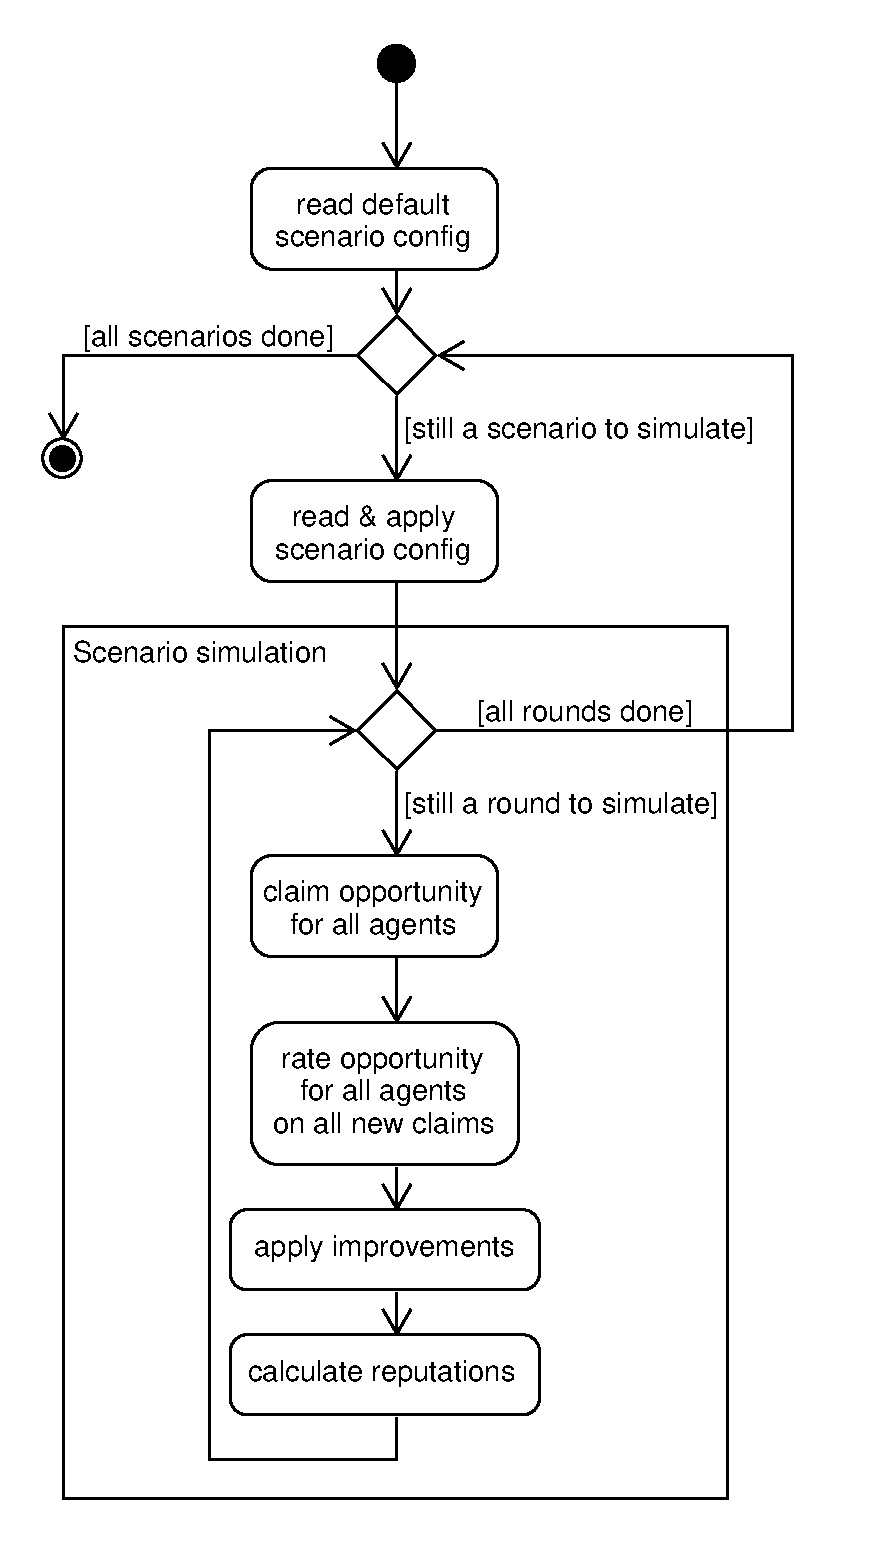
\includegraphics[width=0.75\linewidth]	{../uml/simulation_flow.pdf}
    \caption{
    Simulation flow in Pyrepsys.
    A single simulation unit is the \gls{scenario}.
    Each \gls{scenario} is simulated independently after one another.
    Rounds make up the simulation within a \gls{scenario}.
    Each round consists of four distinct phases: claiming, rating, improvement and reputation calculation.
    The number of rounds is specified in the configuration.
    }
    \label{fig:simulation_flow}
  \end{center}
\end{figure}


\subsection{Claims}
describe claims and what means what

\subsection{Reviews}
describe reviews and what means what

\subsection{Random Number Generation}
reproducability: rng
main chain
sub chains for cases where
- dont know if they need a random
- they need and dont know how many
- they need and dont know what kind (distribution, range etc)
see notes


\subsection{Measuring Claims}\label{sec:approach_measure_claim}
measuring claims

% --------------------------------------------------------------
\section{Reputation Calculation}\label{sec:approach_reputation_calculation}
% --------------------------------------------------------------
BasedOnAvgDifferenceOfClaimsAndReviews
ReputationAverageStrategy

why these two:
	- simple
	- thus easy to know what is happening
	- avg is a common-sense approach that a common user would expect when seeing a star-system
	(even tho that is often not the case in the rep calc, just implied)
	- BasedOnAvgDifferenceOfClaimsAndReviews uniquely uses the author-review system of claim rating
the difference in their interpretation
	ReputationAverageStrategy: a rating becomes a quality of the claimer
	other one: review rates what this claim should have been rated by the author
ability to easily incorporate weights

% --------------------------------------------------------------
\section{Distortion Strategies}\label{sec:distort_strategies}
% --------------------------------------------------------------
% other name: Attack Strategies

\cite{yu_detecting_2003} has the four static in the graph..
static:
"pessimistic" rater (rates in the lower range) bad mouthing
"optimistic" rater (rates in the higher range) ballot stuffing
inverted rating (rates good as bad and vice versa)
random rater (rates random all the time)

user tendentially rating extreme
... conservative
random error rater (occasionally makes a significantly inaccurate rating, most ratings honest to a degree of noise, i.e. not perfect!)
	big inaccuracy e.g. erroneous measurement,sensor
	
Seller sells most products with high quality, but some with low quality for benefit. The honest bad reputation report from victim may be submerged, or be mistakenly regarded as unfair rating. \cite{ping_xu_rating_2005}

	
	
dynamic:
build up honest reputation and attack after that
single out an agent and distort their rating only, honest otherwise
mayb combine negative and positive attacks in collusion scenario, where attackers uprate each other and downrate their target
mayb make difference bw. targeted attack on someone or group and just wrecking havoc on all

individual vs collusion scenarios



% --------------------------------------------------------------
\section{Rating Strategies}\label{sec:approach_rating_strategies}
% --------------------------------------------------------------









% CHAPTER ######################################################################
\chapter{Implementation}\label{chap:implementation}
% ##############################################################################
%Implementation: If you did one, explain all the details here: hardware (chips, buses), OS, compiler, libraries, data structures and their field sizes.

Simulations are done with a custom-made python simulation framework named pyrepsys.
This chapter gives the implementation-specific details of pyrepsys. 
For a conceptual description, see Section~\ref{sec:approach_evaluation_framework}.

Pyrepsys is a one-stop solution for simulating, comparing and evaluating reputation schemes.
Simulation of scenarios is performed on a round-by-round basis.
Shared configuration among scenarios, simulating batches of scenarios in succession and controlled random number generation help compare different scenarios.
Evaluation is aided by metrics.
These can automatically generate graphs and export data from simulations.

Flexibility and extendability are among the main design objectives of pyrepsys.
Variables can be altered in scenario configuration files.
The size and composition of the agent population is customizable.
New agent behaviors, metrics, reputation calculation and imporvement methods can be easily added.

Miscallaneous supportive functionalities are also discussed in this chapter.
A scenario configuration creator can be used to make a batch of scenarios with variations along selected configuration parameters.
Extensive automated self-testing can verify the integrity of the simulation framework if any changes are made.
Finally, profiling and benchmarking tests are provided to identify simulation bottlenecks and measure performance.

Additional references for using Pyrepsys are provided outside this chapter.
For a description of the pyrepsys command-line interface, refer to Appendix~\ref{appendix:cli_invocation}.
A complete list and explanation of possible scenario configuration parameters are found in Appendix~\ref{appendix:scenarios}.
% Finally, information regarding the scenario creator 

TODO: prerequisites, dependencies, tested versions, environment





% --------------------------------------------------------------
\section{Simulation Flow}\label{sec:impl_simulation}
% --------------------------------------------------------------

general simulation flow +flow diag
claiming process
rating process
measuring claims
improvement handling process
reputation calculation (for completeness' sake)

extendable strategies: distort, rate, reputation + metric (adding new ones too?)


% --------------------------------------------------------------
\section{Data Handling}\label{sec:impl_data}
% --------------------------------------------------------------
data structures: agents, claims, reviews (classes) + metrics (as they will)
internal vs ae data storage
precision/resolution domains handling


% --------------------------------------------------------------
\section{Random Number Generation}\label{sec:impl_rng}
% --------------------------------------------------------------



% --------------------------------------------------------------
\section{Results Processing}\label{sec:impl_results_processing}
% --------------------------------------------------------------
After the simulation is finished, Pyrepsys processes the collected data and exports it as graphs or tables.
Collection during sim
events

artifacts
metrics
  graph
  data 
reproc
event based subscribe-notify + uml


% --------------------------------------------------------------
\section{Configuration}\label{sec:impl_config}
% --------------------------------------------------------------
configuration (process)
	where are configs are stored (responsibilities) (config.get, local caches, local configs)
	reading in
	2-leveled: default and active config
	config updated callbacks
	base behaviors
	extended entries / entries extended with settings
CHECK: all big config options covered

mention: scenario creator, link appendix


% --------------------------------------------------------------
\section{Other Facilities}\label{sec:impl_misc}
% --------------------------------------------------------------

Automated Self-Testing
performance
other facilities (logging, error handling, helpers, paths?)


% CHAPTER ######################################################################
\chapter{Evaluation} \label{chap:evaluation}
% ##############################################################################


% --------------------------------------------------------------
\section{Metrics}\label{sec:metrics}
% --------------------------------------------------------------
%Metrics: First define which quantities you will measure and why you chose those.

- reputation
- avg tot claim inaccuracy
- also other metrics from my notebook

% --------------------------------------------------------------
\section{Setup}\label{sec:setup}
% --------------------------------------------------------------
%Setup: Clearly describe which method you use to obtain your values and how the setup looks like. It is probably one of three:
%    Analysis: provide a formal/mathematical analysis of your approach (and related work). Which models / equations do you use? Why? How? 
%    Simulation: Run your approach in a simulation framework. Which simulator (version) runs on which hardware (specs)? Which parameters? Why?
%    Experiment: Measure values from a real implementation. Which devices are used? Conditions? Parameters?

simulation setup -- used settings, scenarios
describe different simulation bundles (of scenarios) and their rationale
why they are interesting and what's expected

% --------------------------------------------------------------
\section{Results}\label{sec:results}
% --------------------------------------------------------------
%Results: visualize your results as graphs and compare to the values of related work.

% --------------------------------------------------------------
\section{Discussion}\label{sec:discussion}
% --------------------------------------------------------------
%Discussion: Explain where, why, and to which extend you have or have not improved over related work. What does this mean for your initial problem question?







% CHAPTER ######################################################################
\chapter{Conclusion} \label{chap:conclusion}
% ##############################################################################
%Conclusion: Summarize main points; formulate key message.
%    Remind the readers what they have read and why it was significant. Don’t give new explanations, just the facts.
%    Repeat the most important result (number!) and what it means for the problem.
 
\lettrine{W}{e} successfully ...




% --------------------------------------------------------------
\section{Outlook}\label{sec:outlook}
% --------------------------------------------------------------

But we still need to ...






\begin{appendix}
\chapter{Scenario Configuration Options}\label{appendix:scenarios}
TODO comprehensive list of all scenario parameters

\chapter{Command Line Interface and Invocation}\label{appendix:cli_invocation}
TODO extensive CLI description

\chapter{Scenario Creator}\label{appendix:sc}
TODO SC desc

\end{appendix}


% Abbreviations
%	\printglossary[type=\acronymtype,title=Abbreviations]

% Glossaries 
\printglossary[type=acronym]       % print only acronyms

\printglossary

%\printglossaries                        % print all glossaries
%\printnoidxglossary[sort=word]
%\printnoidxglossaries


% ##############################################################################

%\nocite{*}   % use this to print all references

% print bibliography
% check if biblatex or legacy bibtex is used
\ifoptionbiblatex
    \printbibliography[heading=bibintoc]              % print BibLaTex bibliography
\else
    \addcontentsline{toc}{chapter}{Bibliography}
    \bibliographystyle{ieeetr}      % bibtex style
    \bibliography{references}       % bibtex library filename(s) WITHOUT extension
\fi


\end{document}


